\documentclass[9pt,conference]{IEEEtran}
\usepackage{cite}
\usepackage{amsmath,amssymb,amsfonts}
\usepackage{multirow}
\usepackage{array}
\usepackage{graphicx}
\usepackage{textcomp}
\usepackage{xcolor}
\usepackage{algorithm}
\usepackage[noend]{algpseudocode}
\usepackage{hhline}
\usepackage{mathrsfs}
\usepackage{float}
\graphicspath{{Figures/}}
\usepackage{epstopdf}
\epstopdfsetup{outdir=./}

\begin{document}

\title{GROUP\_14\_Experiment: 2\\Application of OPAMP (IC741) as Inverting amplifier, Non-inverting amplifier, Differentiator and Integrator}

\author{
    \IEEEauthorblockA{Siddhant Shah (B23334) *, Akash Goel(B23032) †, 
                      Om Maheshwari (B23089) ‡, and Somya Bhadada (B23052) §}
* b23334@students.iitmandi.ac.in \\
† b23032@students.iitmandi.ac.in \\
‡ b23089@students.iitmandi.ac.in \\
§ b23052@students.iitmandi.ac.in}
\date{}

\maketitle


\begin{abstract}
\noindent{This report presents the study and implementation of OPAMP as Inverting amplifier, Non-inverting amplifier, Differentiator and Integrator. The study covers comparison of the graph that we obtained in Lab and the graph that we obtained from LTspice by implmenting the same circuits in it. Also we were given a double differential equation of Vout in terms of Vin so upon solving that we'll get values of Vin and its derivative which we will put in the circuit given and obtain the output waveform through LTspice.}
\end{abstract}

\section{Components Required}
\begin{itemize}
    \item 	{OPAMP IC 741}
    \item 	{Resistors:}
    \begin{itemize}
        \item Two \(1k\Omega\)
        \item One \(10k\Omega\)
    \end{itemize}
    \item 	{Capacitors:}
    \begin{itemize}
        \item Two \(0.01\mu F\)
    \end{itemize}
    \item 	{Programmable DC Power Supply:} Keithley 2231A-30-3
    \item 	{Breadboard}
    \item 	{Digital Storage Oscilloscope (DSO) with Waveform Generator:} Keysight DSOX1102G
    \item 	{Function Generator:} Tektronix AFG1062
    \item 	{Connecting Wires}
    \item 	{Multimeter}
\end{itemize}

\section{Theory}
\noindent{An operational amplifier (op-amp) is a highly versatile, DC-coupled, high-gain electronic voltage amplifier with a differential input and a single-ended output. It forms the core of numerous analog circuits, serving as a fundamental building block in signal processing, control systems, and instrumentation. Op-amps are designed to amplify voltage differences between their inverting ($-$) and non-inverting ($+$) inputs while maintaining high input impedance and low output impedance.}
\subsection{Common Op-Amp Configurations}
\noindent{Op-amps can be configured in various modes depending on the desired operation. The most common configurations include:}

\subsubsection{Inverting Amplifier}
\noindent{Provides phase-inverted amplification with a gain determined by external resistors. It is widely used in audio processing, instrumentation, and active filters.}

\subsubsection{Non-Inverting Amplifier}
\noindent{Maintains the phase of the input signal while amplifying it. This configuration is commonly used in buffer circuits, signal conditioning, and sensor interfacing.}

\subsubsection{Integrator}
\noindent{A fundamental analog computing circuit that performs mathematical integration of the input signal. It acts as a low-pass filter, attenuating high-frequency components and allowing low-frequency signals to pass. Integrators are extensively used in analog computers, function generators, and signal reconstruction in communication systems.}

\subsubsection{Differentiator}
\noindent{A circuit that outputs the derivative of the input signal. It functions as a high-pass filter, amplifying high-frequency signals while attenuating low-frequency components. Differentiators are crucial in edge detection, motion sensing, and high-speed signal processing applications.}

\subsection{Applications of Op-Amp Circuits}
\noindent{Op-amp circuits are widely used in analog and mixed-signal systems due to their precision and adaptability. Some key applications include:}

\subsubsection{Analog-to-Digital (ADC) and Digital-to-Analog Converters (DAC)}
\begin{itemize}
    \item Integrator and differentiator circuits play a vital role in sigma-delta ADCs, modulating signals before conversion.
    \item Op-amp-based sample-and-hold circuits stabilize signals for accurate digital conversion.
\end{itemize}

\subsubsection{Wave-Shaping Circuits}
\begin{itemize}
    \item Integrators and differentiators are used in waveform generators to shape triangular, square, and sinusoidal waveforms.
    \item Charge amplifiers, often built using op-amps, are employed in piezoelectric sensor circuits for measuring dynamic forces.
\end{itemize}

\subsubsection{Control Systems and Feedback Networks}
\begin{itemize}
    \item Op-amps are used in Proportional-Integral-Derivative (PID) controllers for industrial automation and robotics.
    \item They provide active filtering in power electronics and signal conditioning in biomedical applications.
\end{itemize}

\subsubsection{Audio and Communication Systems}
\begin{itemize}
    \item Inverting and non-inverting amplifiers serve as preamplifiers, equalizers, and volume control circuits in audio systems.
    \item Op-amp-based active filters are used in radio-frequency (RF) signal processing and noise reduction applications.
\end{itemize}

\subsection{The IC741 Operational Amplifier}
\noindent{The 741 op-amp is one of the most commonly used general-purpose operational amplifiers, known for its ease of use, reliability, and cost-effectiveness. It features:}
\begin{itemize}
    \item Input offset voltage of a few millivolts, suitable for precision applications.
    \item A unity-gain bandwidth of approximately 1 MHz, making it effective for low-to-moderate frequency applications.
    \item Short-circuit protection, ensuring stable operation under various load conditions.
\end{itemize}

\noindent{Although newer high-performance op-amps with better speed, noise characteristics, and power efficiency are available today, the 741 remains a staple in educational circuits, basic amplifiers, and simple analog computing applications.}\\

\noindent{The Standard Structure of IC741 OPAMP is shown below:}
\begin{figure}[H]
    \centering
    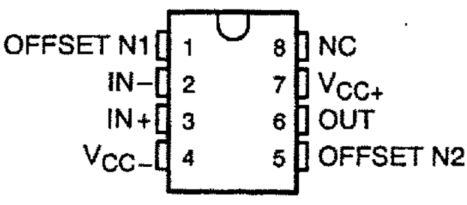
\includegraphics[width=0.7\columnwidth]{IC_741.png}
    \caption{Op-amp Diagram}
    \label{fig:clamper_circuit}
\end{figure}



\section{Observations and Results}
\subsection{Inverting Amplifier}
\begin{itemize}
    \item Implemented a Inverting Amplifier circuit on the breadboard same as the circuit which is given below
\end{itemize}
\begin{figure}[H]
    \centering
    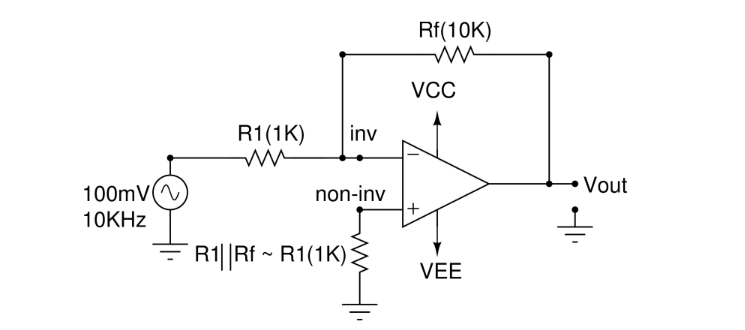
\includegraphics[width=1.0\columnwidth]{inverting_amplifier_circuit.png}
    \caption{Inverting Amplifier Circuit}
    \label{fig:clamper_circuit}
\end{figure}

\begin{figure}[H]
    \centering
    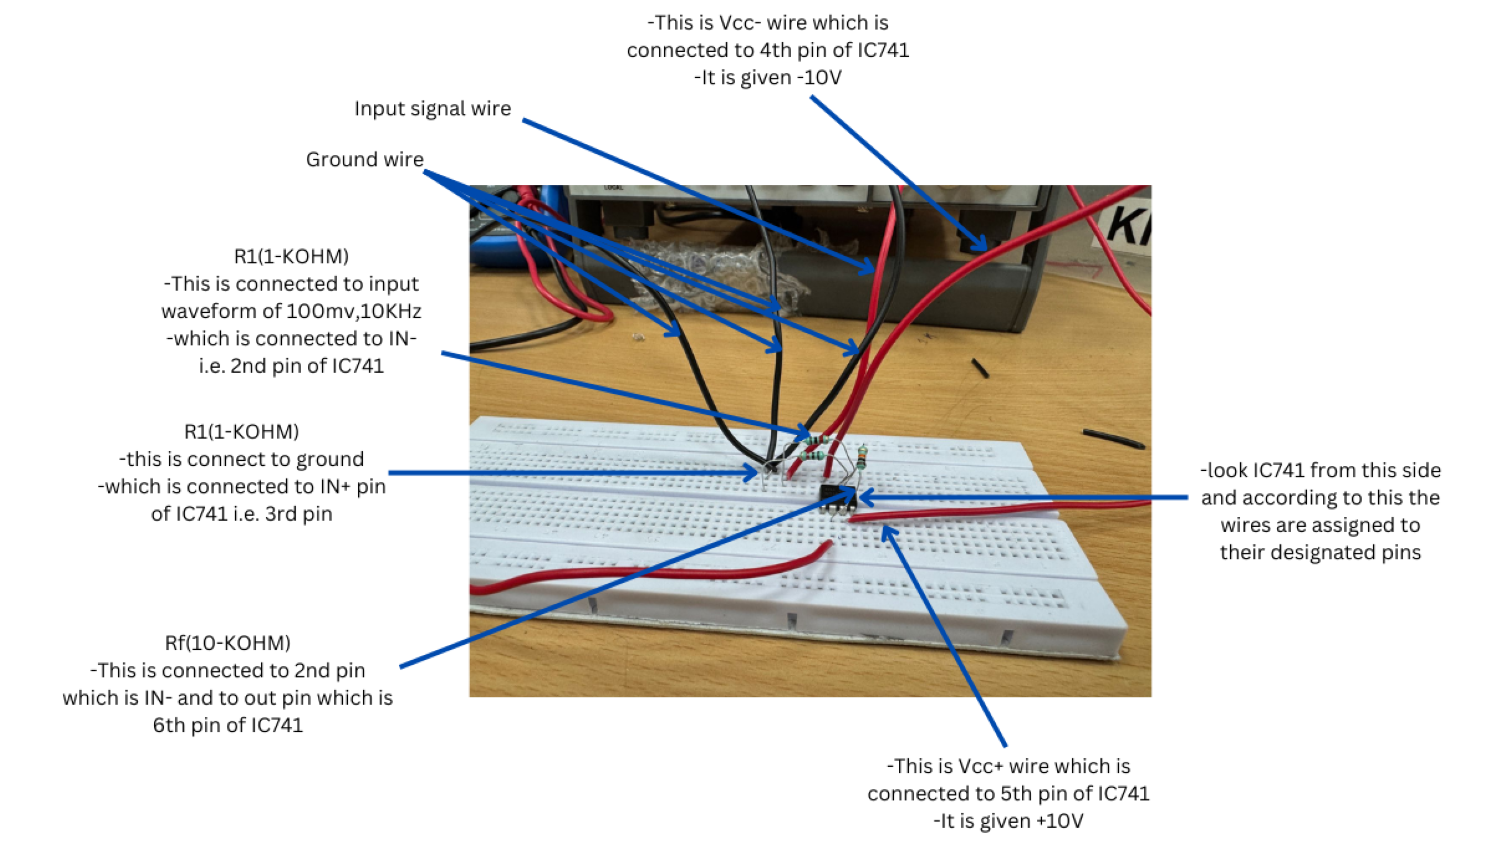
\includegraphics[width=1.0\columnwidth]{inverted_amplifier_circuit_breadboard.png}
    \caption{Inverting Amplifier Circuit Breadboard}
    \label{fig:positive_clamper}
\end{figure}
\begin{itemize}
    \item When an input voltage is applied to the inverting terminal through a resistor, the operational amplifier (op-amp) maintains a virtual ground at the inverting terminal due to the high open-loop gain.
    \item The non-inverting terminal is typically connected to ground, ensuring that the inverting terminal remains at zero volts due to negative feedback.
    \item The input signal passes through the input resistor and reaches the inverting terminal, where it generates a current that flows towards the output through the feedback resistor.
    \item Since no current flows into the op-amp terminals (ideal case), the same current that enters through the input resistor must flow through the feedback resistor.
    \item According to Ohm's Law and Kirchhoff's Current Law (KCL), this results in an output voltage that is inverted and scaled based on the ratio of the feedback resistor to the input resistor.
    \item The gain of the amplifier is given by \( A_v = -\frac{R_f}{R_{1}} \), meaning the output is an amplified and inverted version of the input signal.
    \item As you can see in the graph below, the inverted waveform is amplified and inverted.
\end{itemize}

\begin{figure}[H]
    \centering
    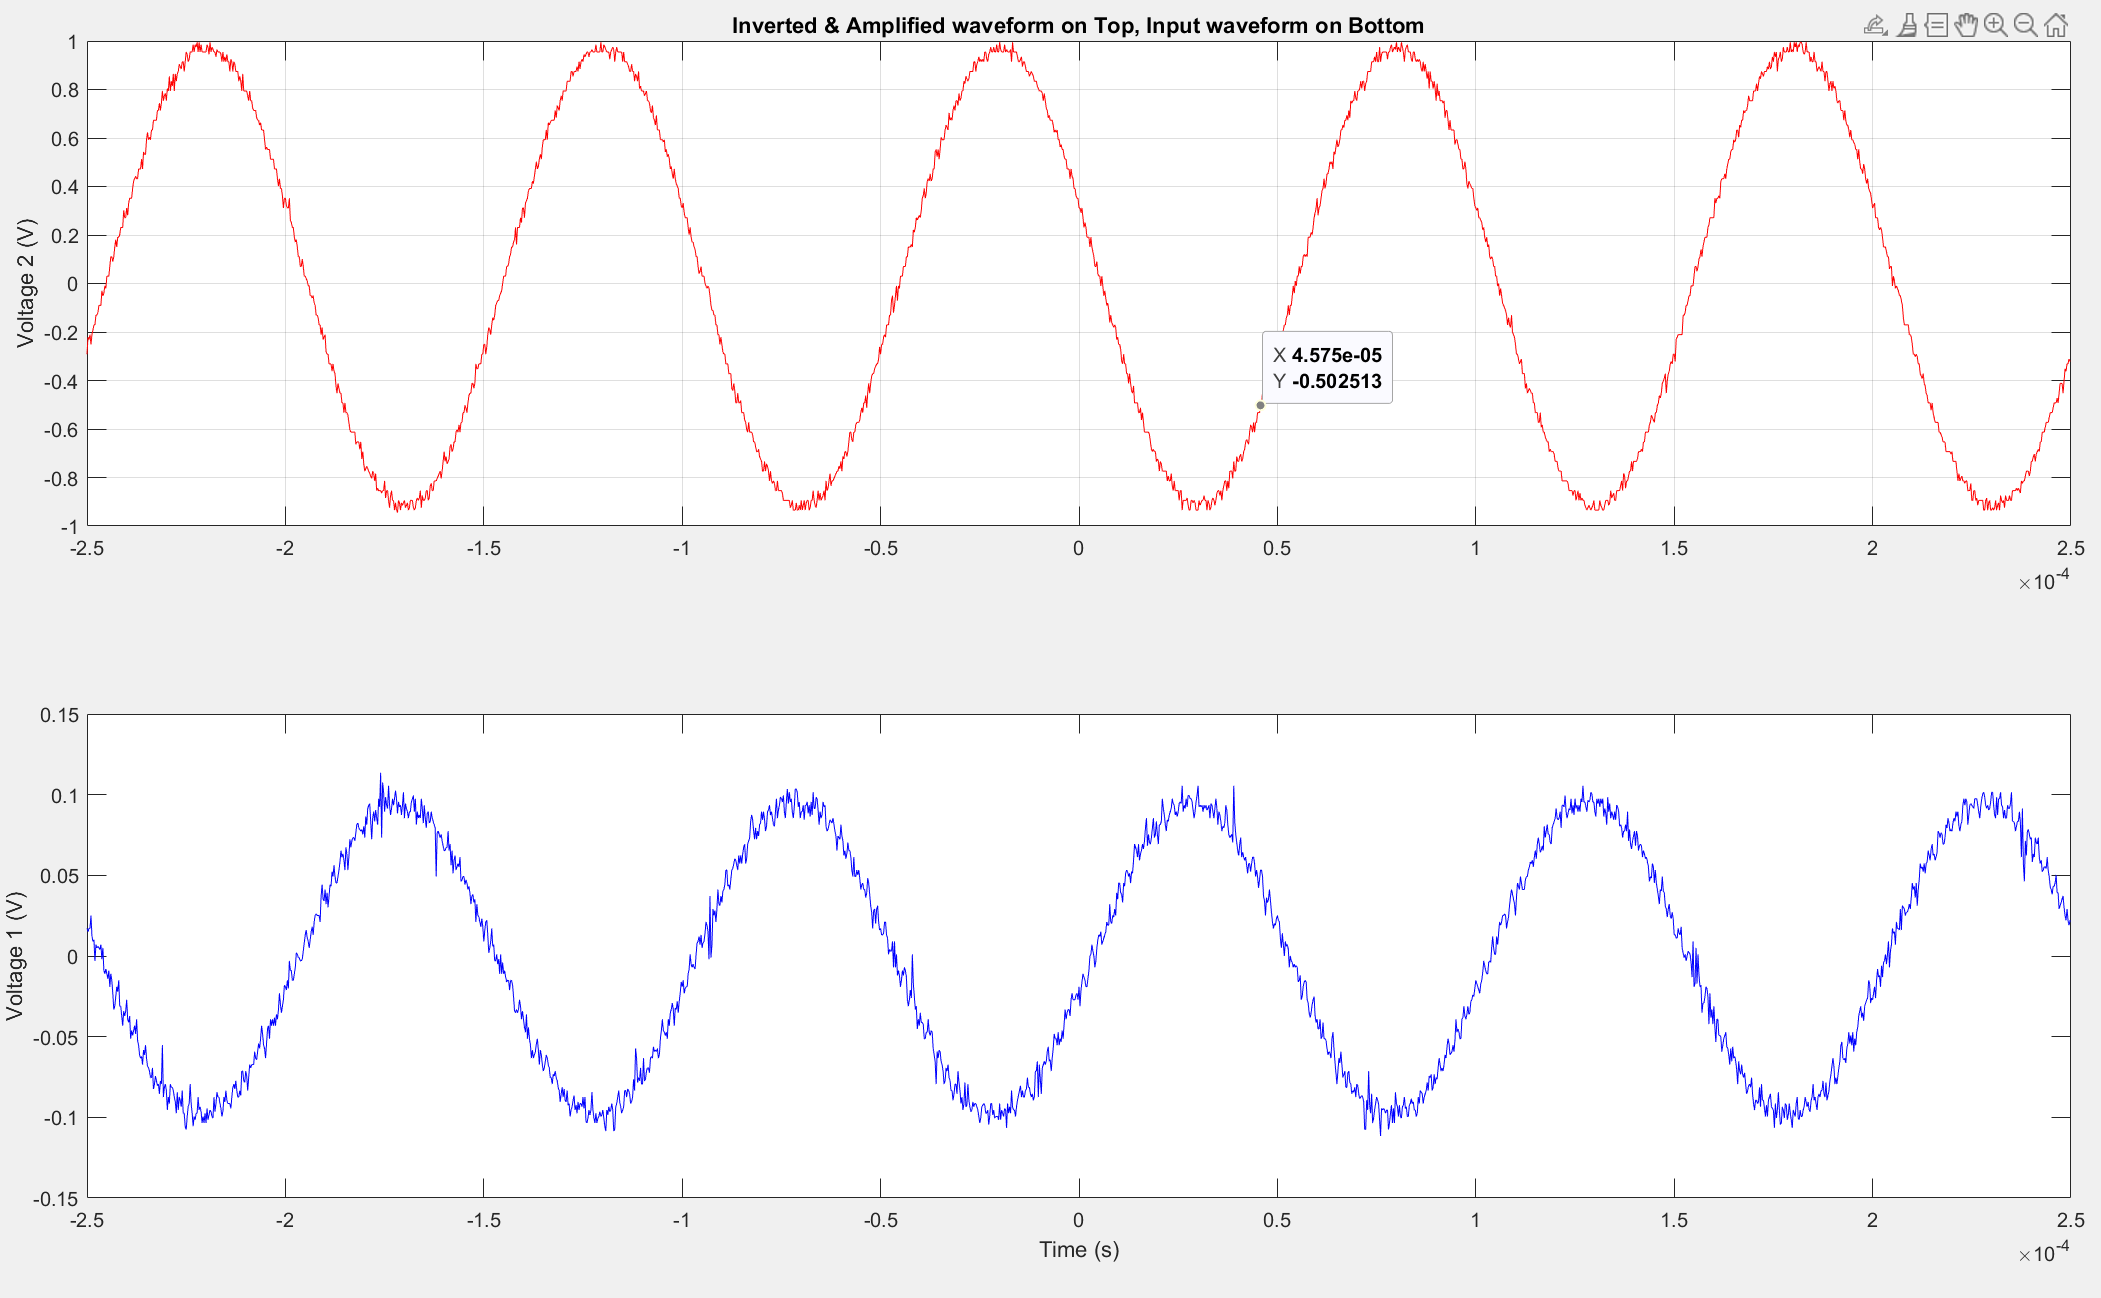
\includegraphics[width=1.0\columnwidth]{inverting_amplifier_graph.png}
    \caption{Inverting Amplifier Circuit Graph(MATLAB)}
    \label{fig:positive_clamper}
\end{figure}

\begin{itemize}
    \item Now if we compare to the LTspice results , you can see the circuit and the graph below . The results which we obtain on LTspice exactly match our Lab output. Hence, The circuit is verified.
\end{itemize}
\begin{figure}[H]
    \centering
    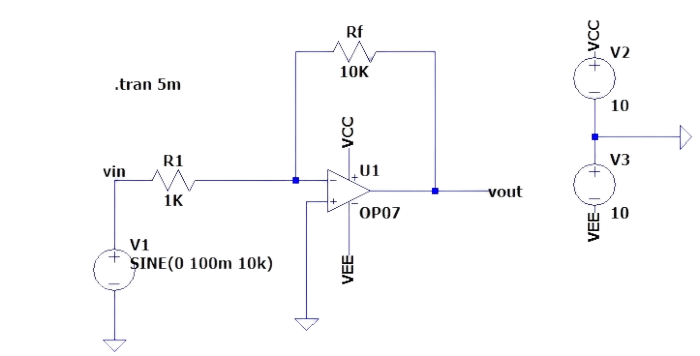
\includegraphics[width=1.0\columnwidth]{LTspice_inverting_circuit.png}
    \caption{LTspice Inverting Amplifier Circuit}
    \label{fig:positive_clamper}
\end{figure}
\begin{figure}[H]
    \centering
    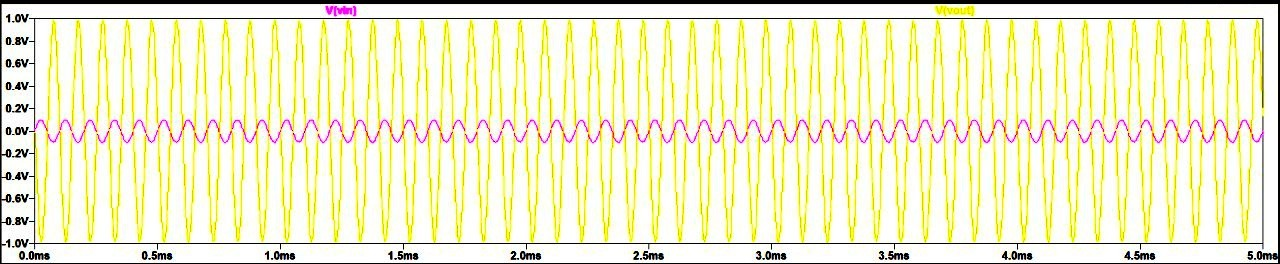
\includegraphics[width=1.0\columnwidth]{LTspice_inverting.jpg}
    \caption{LTspice Inverting Amplifier Circuit Graph}
    \label{fig:positive_clamper}
\end{figure}

\subsection{Non-Inverting Amplifier}
\begin{itemize}
    \item Implemented a Non-Inverting Amplifier circuit on the breadboard same as the circuit which is given below
\end{itemize}
\begin{figure}[H]
    \centering
    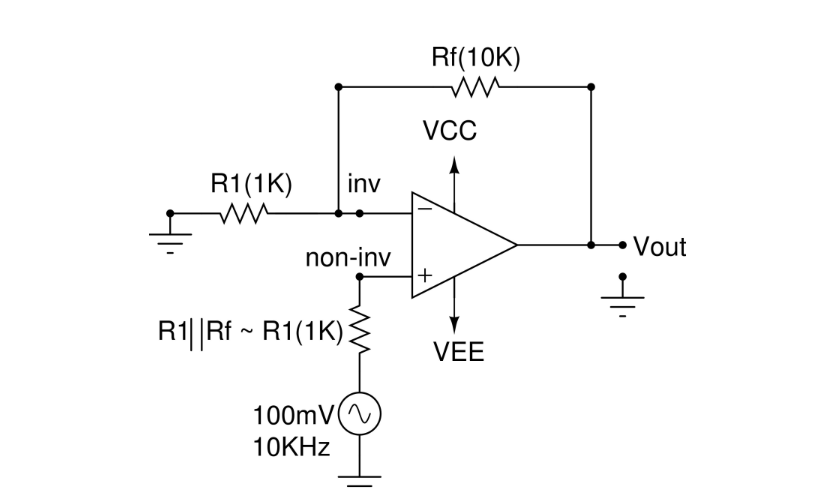
\includegraphics[width=1.0\columnwidth]{non-inverting_amplifier_circuit.png}
    \caption{Non-Inverting Amplifier Circuit}
    \label{fig:clamper_circuit}
\end{figure}

\begin{figure}[H]
    \centering
    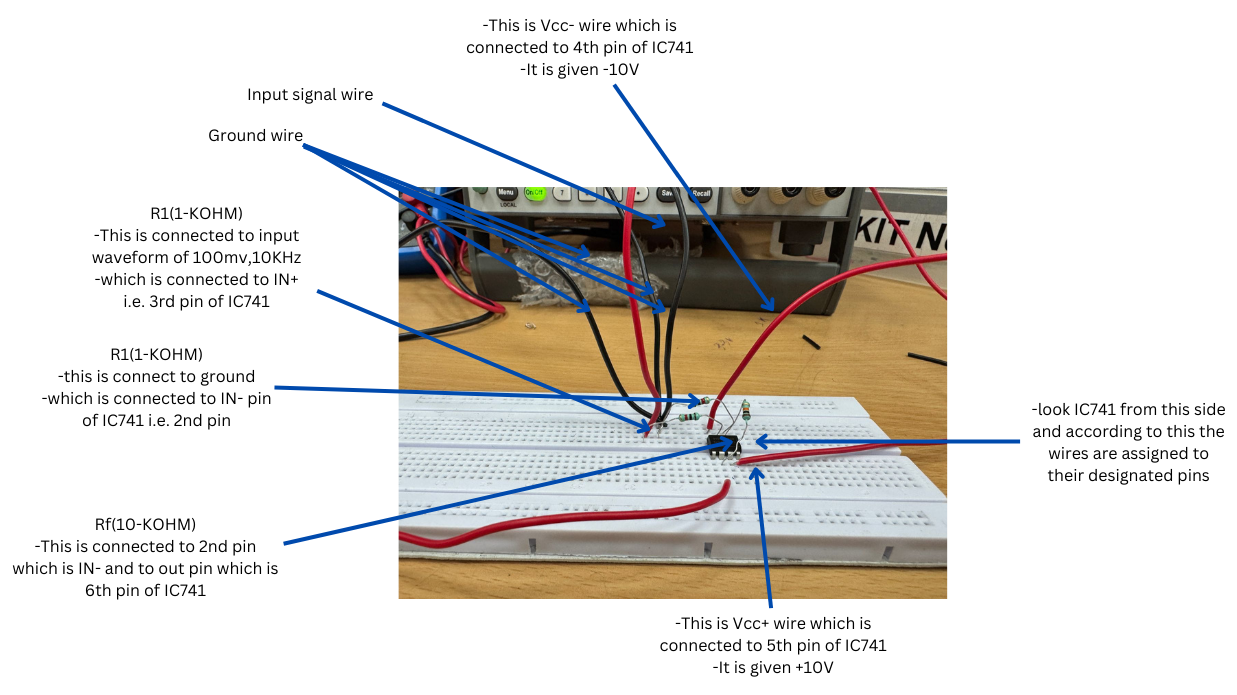
\includegraphics[width=1.0\columnwidth]{Non_inverting_circuit_breadboard.png}
    \caption{Non-Inverting Amplifier Circuit Breadboard}
    \label{fig:positive_clamper}
\end{figure}

\begin{itemize}
    \item When an input voltage is applied to the non-inverting terminal of the operational amplifier (op-amp), the op-amp amplifies the signal while maintaining the same polarity.
    \item The inverting terminal is connected to a voltage divider consisting of a feedback resistor and a resistor to ground, creating a closed-loop feedback system.
    \item Due to the high open-loop gain of the op-amp, the voltage at the inverting terminal is forced to be equal to the voltage at the non-inverting terminal, a concept known as virtual short.
    \item The input signal is not directly affected by the resistor network but influences the voltage at the inverting terminal, which determines the output voltage through the feedback loop.
    \item According to Ohm's Law and Kirchhoff's Voltage Law (KVL), the gain of the amplifier is determined by the ratio of the feedback resistor to the resistor connected to ground.
    \item The voltage gain of the non-inverting amplifier is given by \( A_v = 1 + \frac{R_f}{R_1} \), meaning the output signal is an amplified version of the input signal without inversion.
    \item As you can see in the graph below, the waveform remains in phase with the input but is amplified based on the resistor values.
\end{itemize}

\begin{figure}[H]
    \centering
    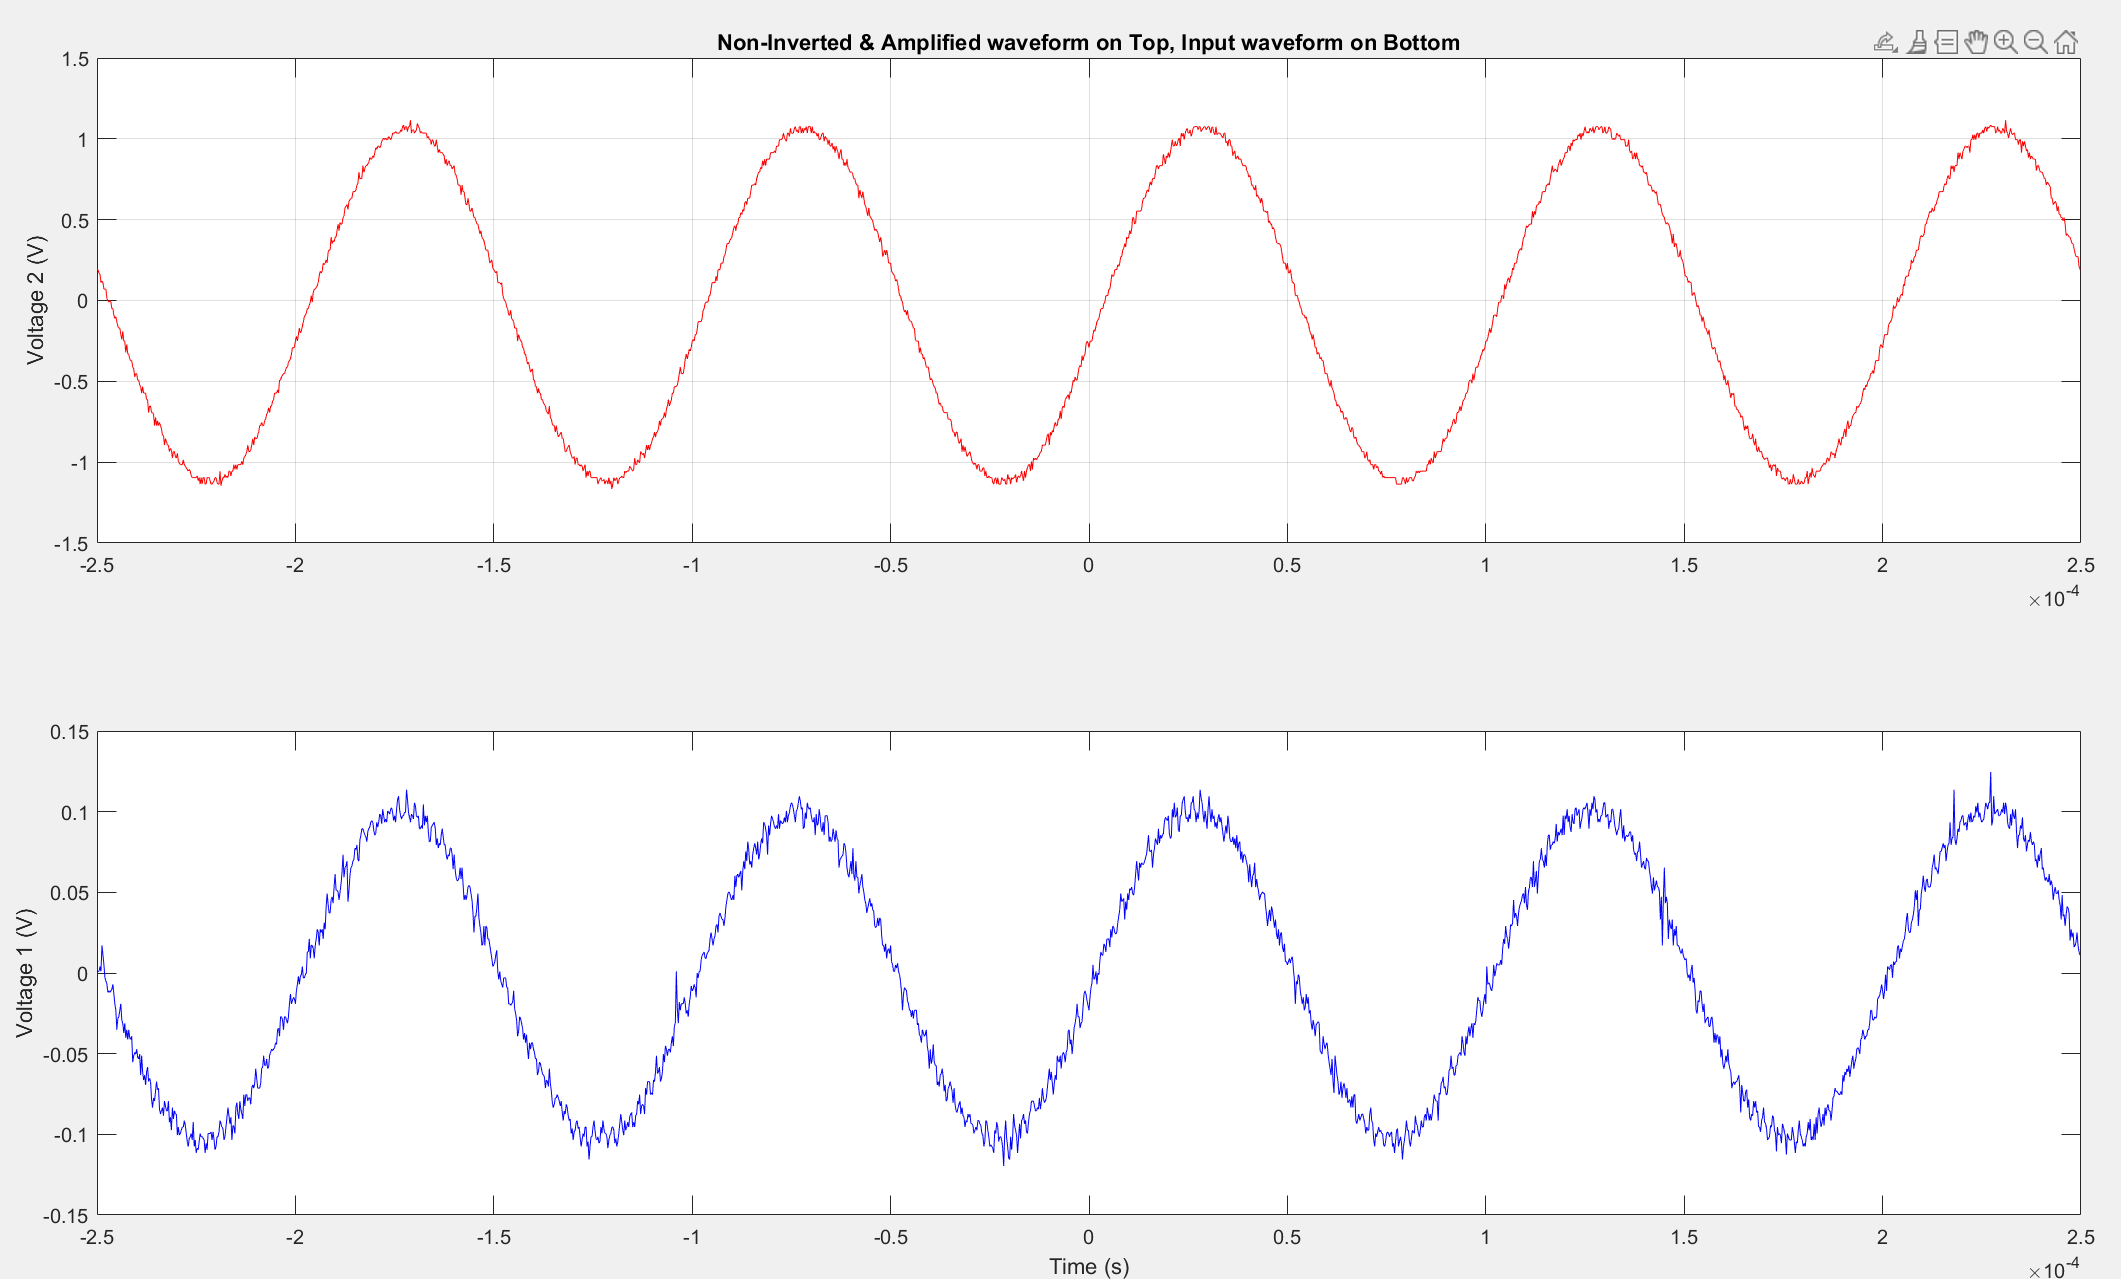
\includegraphics[width=1.0\columnwidth]{Non-inverting_amplifier_graph.png}
    \caption{Non-Inverting Amplifier Circuit Graph(MATLAB)}
    \label{fig:positive_clamper}
\end{figure}

\begin{itemize}
    \item Now if we compare to the LTspice results , you can see the circuit and the graph below . The results which we obtain on LTspice exactly match our Lab output. Hence, The circuit is verified.
\end{itemize}
\begin{figure}[H]
    \centering
    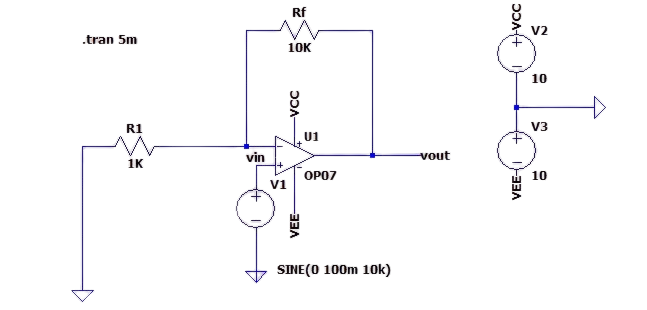
\includegraphics[width=1.0\columnwidth]{LTspice_non-inverting_circuit.png}
    \caption{LTspice Non-Inverting Amplifier Circuit}
    \label{fig:positive_clamper}
\end{figure}
\begin{figure}[H]
    \centering
    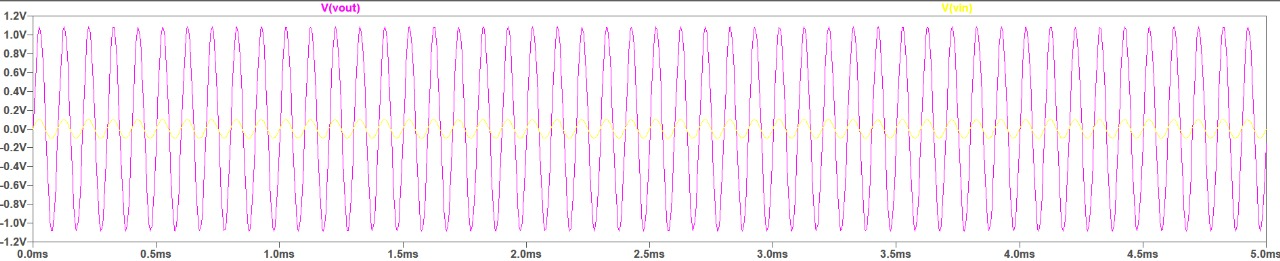
\includegraphics[width=1.0\columnwidth]{LTspice_non-inverting.png}
    \caption{LTspice Non-Inverting Amplifier Circuit Graph}
    \label{fig:positive_clamper}
\end{figure}

\subsection{Integrator}
\begin{itemize}
    \item Implemented a Integrator circuit on the breadboard same as the circuit which is given below
\end{itemize}
\begin{figure}[H]
    \centering
    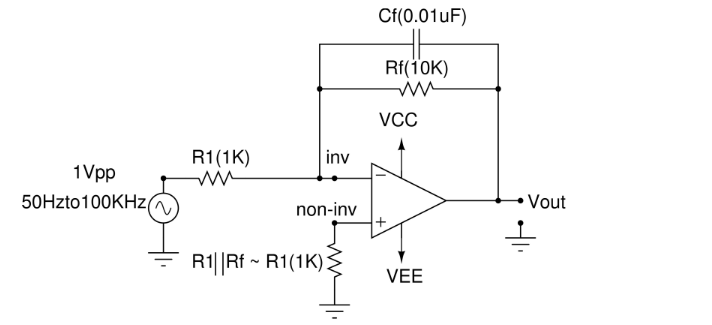
\includegraphics[width=1.0\columnwidth]{Integrator_circuit.png}
    \caption{Integrator Circuit}
    \label{fig:clamper_circuit}
\end{figure}

\begin{itemize}
    \item When an input voltage is applied to the inverting terminal of the operational amplifier (op-amp), the circuit behaves as an integrator, producing an output proportional to the time integral of the input signal.
    \item The circuit consists of a feedback capacitor instead of a resistor, and an input resistor that allows current to flow based on the input voltage.
    \item Due to the high open-loop gain of the op-amp, the voltage at the inverting terminal is maintained at virtual ground, meaning it remains at approximately zero volts.
    \item The input voltage causes a current to flow through the input resistor, which in turn charges or discharges the capacitor, influencing the output voltage.
    \item According to Kirchhoff’s Current Law (KCL), the current through the input resistor is equal to the current through the capacitor, leading to an integration operation on the input signal.
    \item The output voltage is given by the formula:  
      \[
      V_{\text{out}} = -\frac{1}{RC} \int V_{\text{in}} \, dt
      \]
      meaning the circuit integrates the input voltage over time with a scaling factor of \( 1/RC \).
    \item As you can see in the graph below, when a sine input is applied, the output waveform exhibits a cosine signal, demonstrating the integration behavior.
\end{itemize}


\begin{figure}[H]
    \centering
    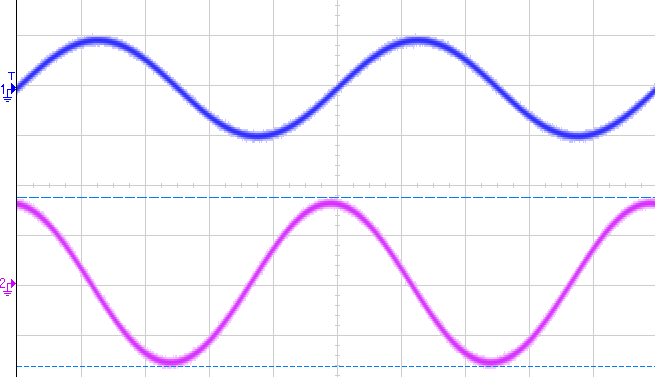
\includegraphics[width=1.0\columnwidth]{Integrator_Output.png}
    \caption{Integrator Output Graph(MATLAB)}
    \label{fig:positive_clamper}
\end{figure}


\begin{figure}[H]
    \centering
    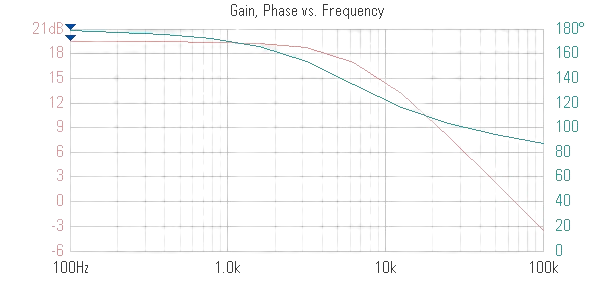
\includegraphics[width=1.0\columnwidth]{Integrator_Frequency_Response.png}
    \caption{Integrator Frequency Response Graph}
    \label{fig:positive_clamper}
\end{figure}

\begin{itemize}
    \item Now if we compare to the LTspice results , you can see the circuit and the graph below . The results which we obtain on LTspice exactly match our Lab output. Hence, The circuit is verified.
\end{itemize}
\begin{figure}[H]
    \centering
    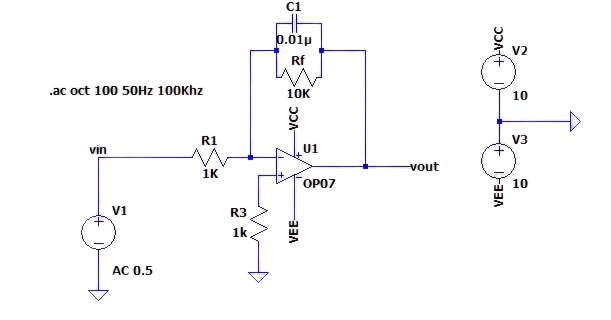
\includegraphics[width=1.0\columnwidth]{LTspice_Integrator.png}
    \caption{LTspice Integrator Circuit}
    \label{fig:positive_clamper}
\end{figure}
\begin{figure}[H]
    \centering
    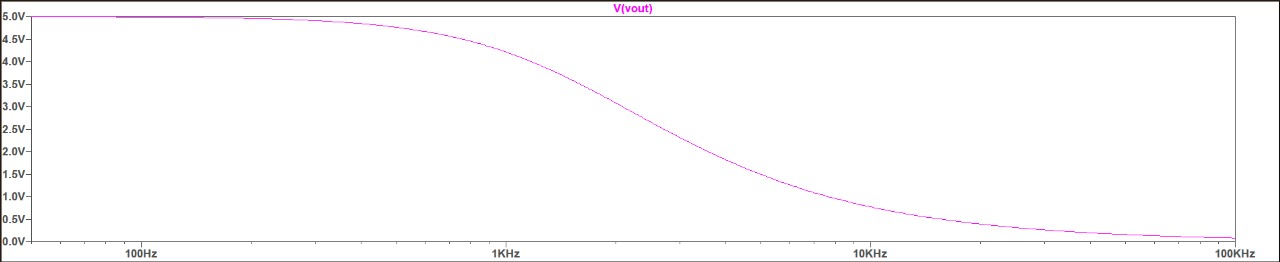
\includegraphics[width=1.0\columnwidth]{LTspice_Integrator_graph.png}
    \caption{LTspice Integrator Circuit Graph}
    \label{fig:positive_clamper}
\end{figure}


\subsection{Differentiator}
\begin{itemize}
    \item Implemented a Differentiator circuit on the breadboard same as the circuit which is given below
\end{itemize}
\begin{figure}[H]
    \centering
    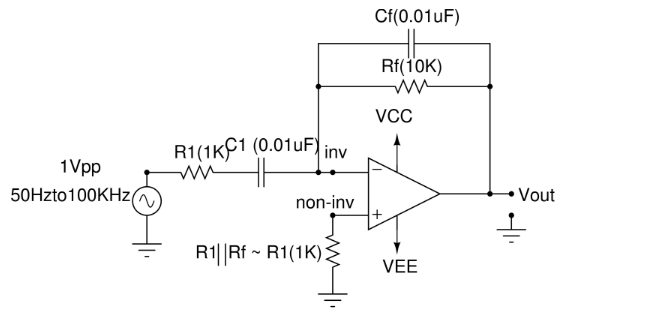
\includegraphics[width=1.0\columnwidth]{Differentiator_circuit.png}
    \caption{Differentiator Circuit}
    \label{fig:clamper_circuit}
\end{figure}

\begin{itemize}
    \item When an input voltage is applied to the inverting terminal of the operational amplifier (op-amp), the circuit behaves as a differentiator, producing an output proportional to the rate of change of the input signal.
    \item The circuit consists of a capacitor in series with the input and a feedback resistor connected from the output to the inverting terminal.
    \item Due to the high open-loop gain of the op-amp, the voltage at the inverting terminal is maintained at virtual ground, meaning it remains at approximately zero volts.
    \item When an input signal is applied, the capacitor allows current to flow based on the rate of change of the input voltage, as capacitors react to changes in voltage rather than steady-state values.
    \item According to Kirchhoff’s Current Law (KCL), the current through the capacitor is proportional to the time derivative of the input voltage and flows through the feedback resistor, generating the output voltage.
    \item The output voltage is given by the formula:  
      \[
      V_{\text{out}} = -RC \frac{dV_{\text{in}}}{dt}
      \]
      meaning the circuit differentiates the input signal over time with a scaling factor of \( RC \).
    \item As you can see in the graph below, when a step input(In the circuit you might be seeing that we gave input signal as sine wave , but while performing actually we are giving Square pulse) is applied, the output waveform exhibits a sharp pulse, demonstrating the differentiation behavior.
\end{itemize}


\begin{figure}[H]
    \centering
    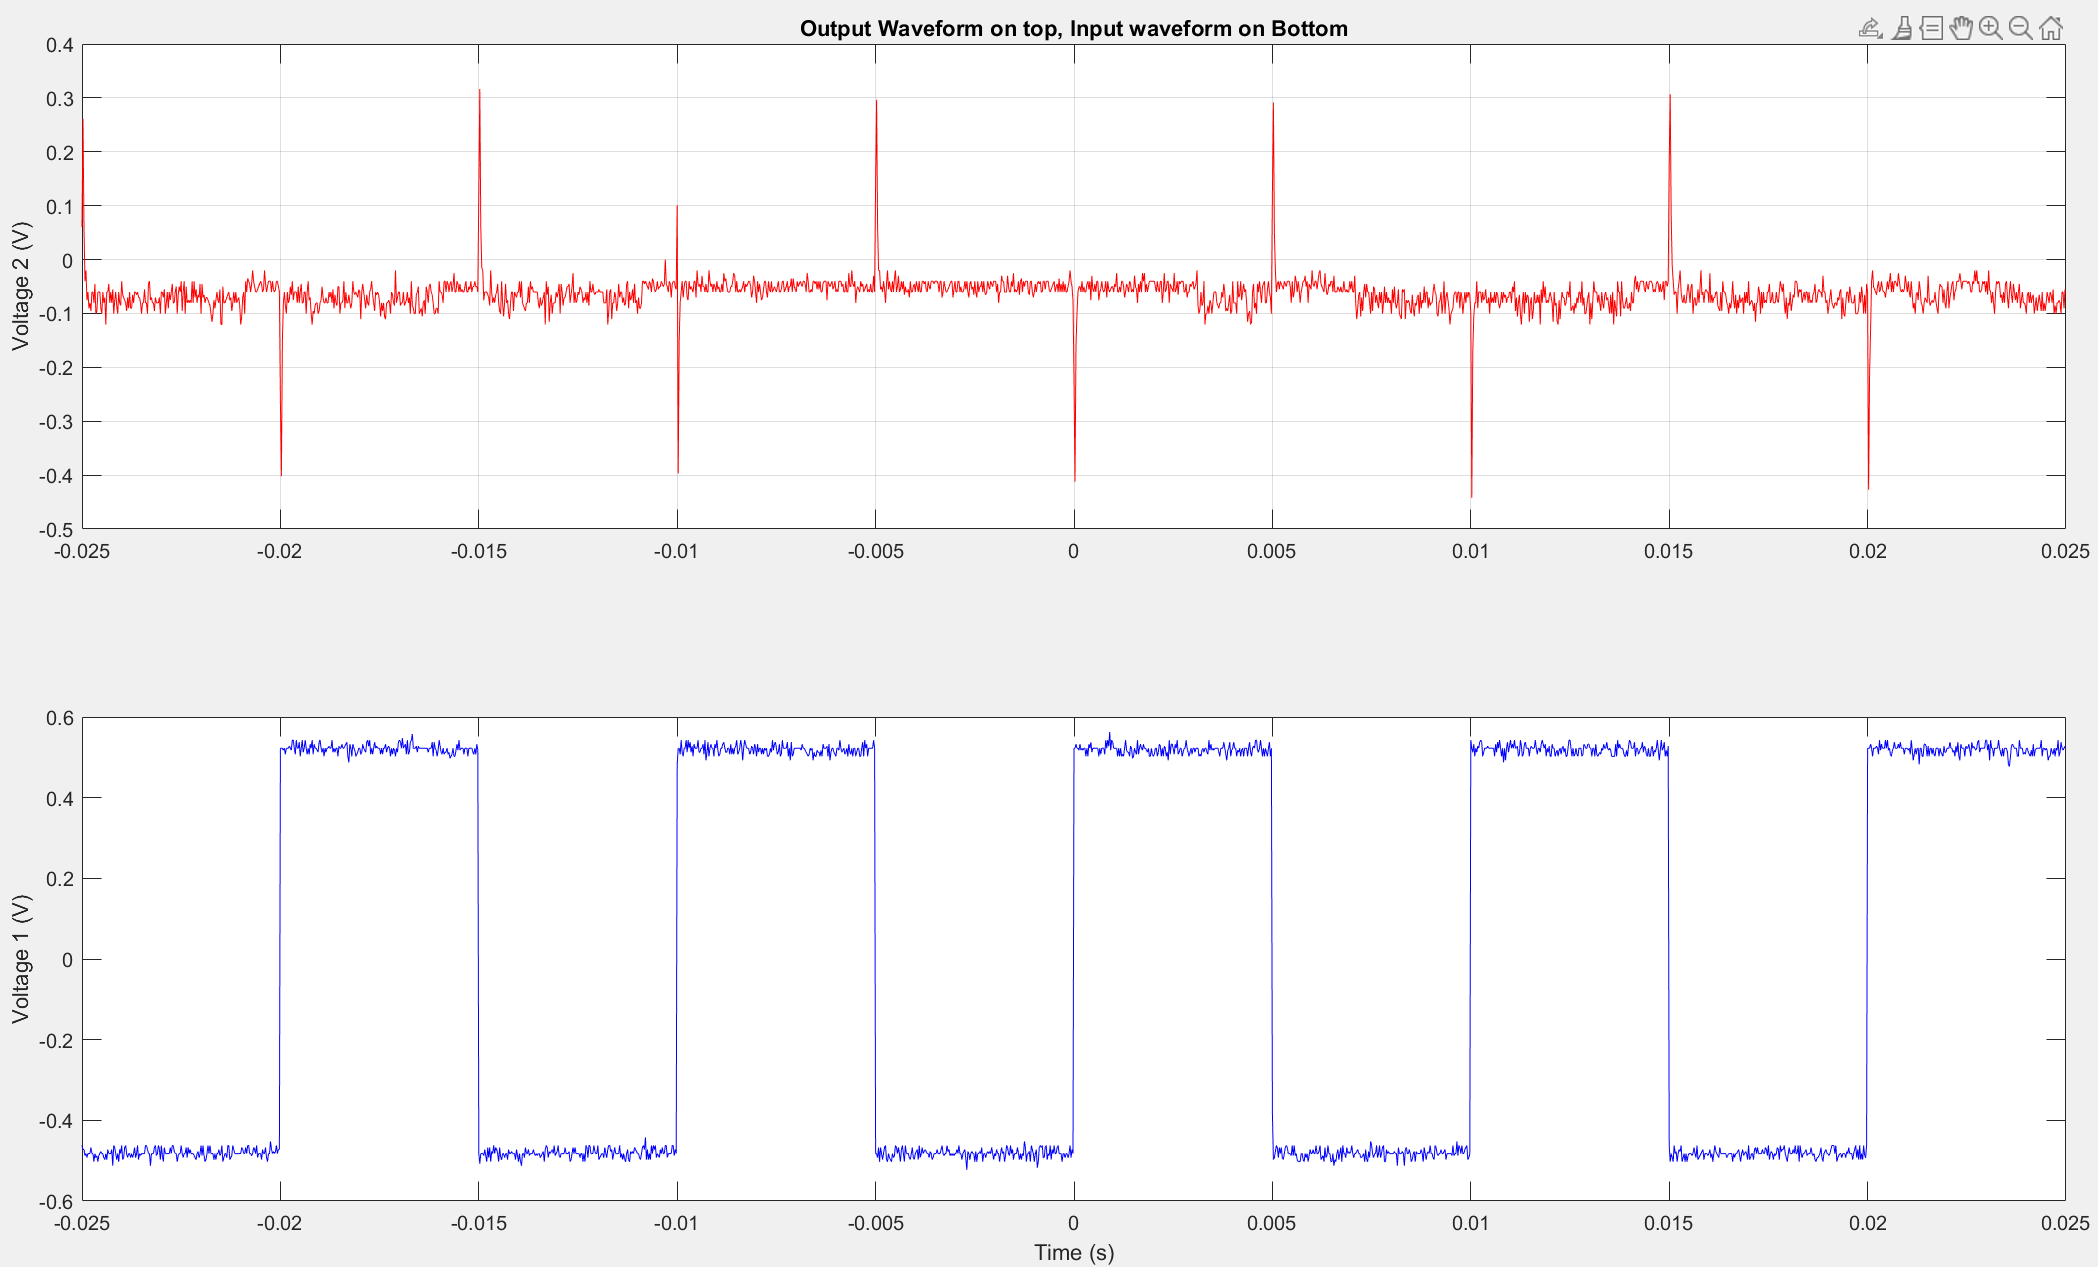
\includegraphics[width=1.0\columnwidth]{Differentiator_Output_graph.png}
    \caption{Differentiator Output Graph(MATLAB)}
    \label{fig:positive_clamper}
\end{figure}
\begin{figure}[H]
    \centering
    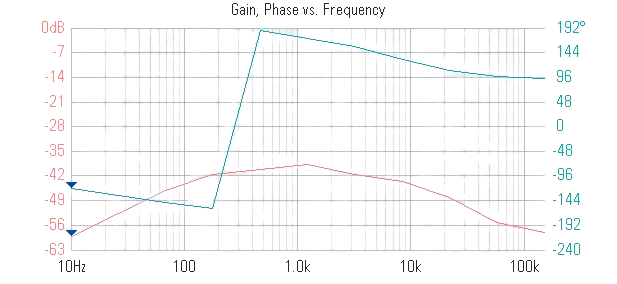
\includegraphics[width=1.0\columnwidth]{Differentiator_Frequency_response_graph.png}
    \caption{Differentiator Frequency response Graph}
    \label{fig:positive_clamper}
\end{figure}

\begin{itemize}
    \item Now if we compare to the LTspice results , you can see the circuit and the graph below . The results which we obtain on LTspice exactly match our Lab output. Hence, The circuit is verified.(Note: We have taken input as sine waveform for LTspice because couldn't implement with square waveform(some issue with LTspice))
\end{itemize}
\begin{figure}[H]
    \centering
    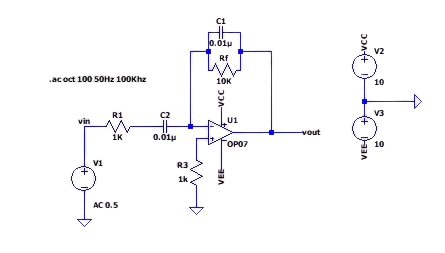
\includegraphics[width=1.0\columnwidth]{LTspice_Differentiator.png}
    \caption{LTspice Differentiator Circuit}
    \label{fig:positive_clamper}
\end{figure}
\begin{figure}[H]
    \centering
    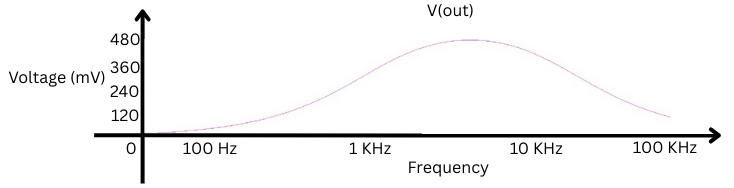
\includegraphics[width=1.0\columnwidth]{LTspice_Differentiator_graph.png}
    \caption{LTspice Differentiator Circuit Graph}
    \label{fig:positive_clamper}
\end{figure}

\subsection{Bonus Question}
\begin{itemize}
    \item We were given a second-order differential equation for \( V_{\text{out}} \) in terms of \( V_{\text{in}} \). Our task was to solve this equation and determine the values of \( V_{\text{in}} \) and its derivative. Based on this, we calculated the appropriate resistor and capacitor values using the concept of a differential circuit.
    \item After solving the circuit, we obtained the following component values:
    \begin{itemize}
        \item Resistors:  
        \( R_1 = 10k\Omega \), \( R_2 = 500\Omega \), \( R_3 = 3.33k\Omega \),  
        \( R_4 = 55.56k\Omega \), \( R_5 = 55.56k\Omega \), \( R_6 = 10k\Omega \)
        \item Feedback Resistors:  
        \( R_{f1} = 10k\Omega \), \( R_{f2} = 10k\Omega \),  
        \( R_{f3} = 10k\Omega \), \( R_{f4} = 10k\Omega \), \( R_{f5} = 10k\Omega \)
        \item Capacitors:  
        \( C_1 = 1\mu F \), \( C_2 = 1\mu F \)
    \end{itemize}
\end{itemize}
\begin{figure}[H]
    \centering
    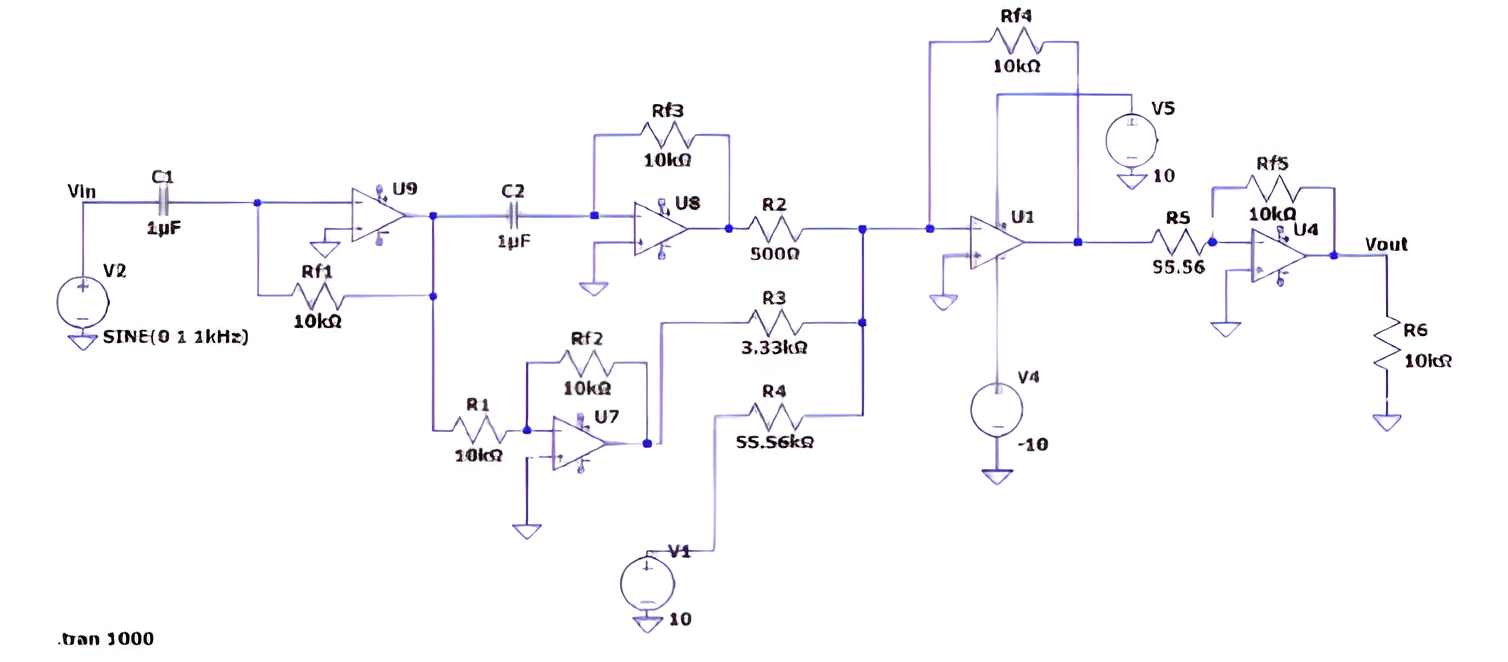
\includegraphics[width=1.0\columnwidth]{Bonus_circuit.png}
    \caption{LTspice Circuit Diagram}
    \label{fig:positive_clamper}
\end{figure}
\begin{figure}[H]
    \centering
    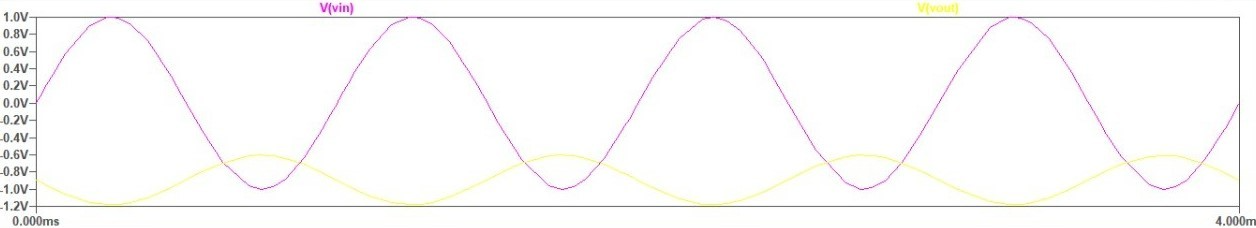
\includegraphics[width=1.0\columnwidth]{Bonus_graph.png}
    \caption{LTspice Graph}
    \label{fig:positive_clamper}
\end{figure}


\section{Discussion}
\begin{itemize}
    \item The experimental implementation of inverting, non-inverting, integrator, and differentiator circuits using operational amplifiers (op-amps) demonstrated expected signal behavior with minor deviations from theoretical values.
    \item The key factors influencing circuit performance include:
    \begin{itemize}
        \item Op-Amp Offset Voltage and Bias Current: Real op-amps exhibit small input offset voltages and bias currents, leading to slight deviations in output voltage.
        \item Finite Open-Loop Gain: Although op-amps are assumed to have infinite gain in theoretical calculations, practical devices have a finite open-loop gain, affecting accuracy.
        \item Component Tolerances: Resistor and capacitor values have manufacturing tolerances (typically \(\pm 5\%\) or \(\pm 1\%\)), which affect gain calculations and time-constant accuracy.
        \item Frequency Response Limitations: The integrator and differentiator circuits depend on frequency; at very high frequencies, phase shifts and attenuation effects were observed due to op-amp bandwidth limitations.
        \item Parasitic Capacitance and Inductance: PCB traces, breadboard wiring, and component leads introduce unwanted parasitic effects that can alter circuit behavior, particularly in high-frequency signals.
        \item Saturation and Slew Rate Limitation: When high-amplitude signals were applied, op-amp output saturation and limited slew rate affected the accuracy of waveform reproduction.
        \item Power Supply Variations: Small fluctuations in the dual power supply affected the op-amp’s ability to maintain an accurate virtual ground and stable output.
        \item Measurement Errors: The use of multimeters and oscilloscopes introduced minor inaccuracies due to probe impedance and signal attenuation.
    \end{itemize}
\end{itemize}

\section{Conclusion}
\noindent{The implementation of inverting, non-inverting, integrator, and differentiator circuits using operational amplifiers was successfully carried out. The observed results closely followed theoretical expectations, with minor deviations due to real-world circuit limitations such as op-amp non-idealities, component tolerances, and parasitic effects. Despite these challenges, the fundamental working principles of each configuration were verified experimentally.}


\section{References}
\begin{enumerate}
    \item Fundamentals of Microelectronics by Behzad Razavi
    \item Microelectronic circuits by Adel Sedra and Kenneth Smith
\end{enumerate}

\end{document}
